\chapter{Análisis}
En este capítulo se describen los requerimientos para el funcionamiento del sistema, un paso crucial para asegurar que la solución final satisfaga las necesidades de los usuarios. Además, se detallan los componentes de hardware y software necesarios para su desarrollo e implementación.

\section{Análisis de Requerimientos del Sistema}
Se presenta un desglose de las capacidades principales del sistema, visualizadas mediante diversas representaciones, como tablas de requerimientos, diagrama de casos de uso y otros elementos complementarios.

\subsection{Requerimientos Funcionales (RF)} \label{sec:requerimientos_funcionales}


Los requerimientos del sistema, derivados del análisis realizado de las necesidades funcionales, se detallan en las Tablas 4.1 a 4.12. Estos requerimientos se centran en las funcionalidades que permiten la interacción del usuario con el sistema para el reconocimiento y la interpretación de la Lengua de Señas Mexicana (LSM). A continuación, se presentan estos requerimientos de manera organizada:

\begin{table}[H]
    \centering
    \begin{tabular}{|p{0.3\linewidth}|p{0.6\linewidth}|}
        \hline
        \textbf{Identificación del requerimiento} & RF01 \\
        \hline
        \textbf{Nombre del requerimiento} & Registro de Usuario \\
        \hline
        \textbf{Definición del requerimiento} & El sistema permite registrar a un usuario que emitirá muestras. \\
        \hline
        \textbf{Descripción del requerimiento} & El sistema permite que el usuario señante se registre ingresando su correo y contraseña. \\
        \hline
        \textbf{Precondiciones requeridas} & El sistema tiene habilitadas las opciones de registro de usuario. \\
        \hline
        \textbf{Prioridad del requerimiento} & Alta \\
        \hline
    \end{tabular}
    \caption{Requerimiento: Registro de Usuario}
    \label{tab:rf-registro-usuario}
\end{table}

\begin{table}[H]
    \centering
    \begin{tabular}{|p{0.3\linewidth}|p{0.6\linewidth}|}
        \hline
        \textbf{Identificación del requerimiento} & RF02 \\
        \hline
        \textbf{Nombre del requerimiento} & Inicio de la Aplicación y del Sistema \\
        \hline
        \textbf{Definición del requerimiento} & El sistema permite iniciar la plataforma correctamente para que el usuario pueda interactuar con la aplicación. \\
        \hline
        \textbf{Descripción del requerimiento} & El usuario puede abrir la aplicación, la cual carga y prepara todos los componentes necesarios para comenzar la captura de señas y la interacción. \\
        \hline
        \textbf{Precondiciones requeridas} & El sistema está instalado y operativo en el dispositivo del usuario. \\
        \hline
        \textbf{Prioridad del requerimiento} & Alta \\
        \hline
    \end{tabular}
    \caption{Requerimiento: Inicio de la Aplicación y del Sistema}
    \label{tab:rf-inicio-app}
\end{table}

\begin{table}[H]
    \centering
    \begin{tabular}{|p{0.3\linewidth}|p{0.6\linewidth}|}
        \hline
        \textbf{Identificación del requerimiento} & RF03 \\
        \hline
        \textbf{Nombre del requerimiento} & Login y Autenticación de Credenciales \\
        \hline
        \textbf{Definición del requerimiento} & El sistema permite que los usuarios inicien sesión y autentiquen sus credenciales. \\
        \hline
        \textbf{Descripción del requerimiento} & El sistema permite autenticar al usuario verificando su correo y contraseña contra la base de datos de usuarios para asegurar que los datos persistan y que el acceso sea seguro. \\
        \hline
        \textbf{Precondiciones requeridas} & El usuario fue registrado previamente en el sistema. \\
        \hline
        \textbf{Prioridad del requerimiento} & Alta \\
        \hline
    \end{tabular}
    \caption{Requerimiento: Login y Autenticación}
    \label{tab:rf-login}
\end{table}

\begin{table}[H]
    \centering
    \begin{tabular}{|p{0.3\linewidth}|p{0.6\linewidth}|}
        \hline
        \textbf{Identificación del requerimiento} & RF04 \\
        \hline
        \textbf{Nombre del requerimiento} & Perfil \\
        \hline
        \textbf{Definición del requerimiento} & El sistema permite al usuario gestionar su perfil. \\
        \hline
        \textbf{Descripción del requerimiento} & El usuario puede ver y actualizar sus datos personales, como nombre, correo y foto de perfil. \\
        \hline
        \textbf{Precondiciones requeridas} & El usuario ha iniciado sesión correctamente. \\
        \hline
        \textbf{Prioridad del requerimiento} & Alta \\
        \hline
    \end{tabular}
    \caption{Requerimiento: Perfil}
    \label{tab:rf-perfil}
\end{table}

\begin{table}[H]
    \centering
    \begin{tabular}{|p{0.3\linewidth}|p{0.6\linewidth}|}
        \hline
        \textbf{Identificación del requerimiento} & RF05 \\
        \hline
        \textbf{Nombre del requerimiento} & Destacados \\
        \hline
        \textbf{Definición del requerimiento} & Ver nombre de los usuarios destacados (destacan por la cantidad de señas que emiten). \\
        \hline
        \textbf{Descripción del requerimiento} & El sistema permite al SEÑANTE ver la lista de usuarios que más han emitido muestras de señas para el sistema. \\
        \hline
        \textbf{Precondiciones requeridas} & El usuario señante está autenticado. \\
        \hline
        \textbf{Prioridad del requerimiento} & Media \\
        \hline
    \end{tabular}
    \caption{Requerimiento: Destacados}
    \label{tab:rf-destacados-revision}
\end{table}

\begin{table}[H]
    \centering
    \begin{tabular}{|p{0.3\linewidth}|p{0.6\linewidth}|}
        \hline
        \textbf{Identificación del requerimiento} & RF06 \\
        \hline
        \textbf{Nombre del requerimiento} & DLM (Ver Información de la Seña) \\
        \hline
        \textbf{Definición del requerimiento} & El sistema permite al usuario ver información detallada de la seña seleccionada. \\
        \hline
        \textbf{Descripción del requerimiento} & El usuario puede acceder a información completa de una seña específica que persista en el sistema. \\
        \hline
        \textbf{Precondiciones requeridas} & El usuario está autenticado. La seña debe existir en el sistema. \\
        \hline
        \textbf{Prioridad del requerimiento} & Alta \\
        \hline
    \end{tabular}
    \caption{Requerimiento: DLM Ver Información de la Seña}
    \label{tab:rf-dlm-ver-informacion}
\end{table}

\begin{table}[H]
    \centering
    \begin{tabular}{|p{0.3\linewidth}|p{0.6\linewidth}|}
        \hline
        \textbf{Identificación del requerimiento} & RF07 \\
        \hline
        \textbf{Nombre del requerimiento} & Captura de Seña para Identificación \\
        \hline
        \textbf{Definición del requerimiento} & El sistema permite la captura de una seña para su posterior identificación. \\
        \hline
        \textbf{Descripción del requerimiento} & El usuario puede capturar una seña y el sistema la procesa para intentar identificarla. \\
        \hline
        \textbf{Precondiciones requeridas} & El sistema tiene la capacidad de procesar secuencias de video o imágenes. \\
        \hline
        \textbf{Prioridad del requerimiento} & Alta \\
        \hline
    \end{tabular}
    \caption{Requerimiento: Captura de Seña para Identificación}
    \label{tab:rf-captura-sena-identificar}
\end{table}

\begin{table}[H]
    \centering
    \begin{tabular}{|p{0.3\linewidth}|p{0.6\linewidth}|}
        \hline
        \textbf{Identificación del requerimiento} & RF08 \\
        \hline
        \textbf{Nombre del requerimiento} & Reconocimiento de Seña \\
        \hline
        \textbf{Definición del requerimiento} & El sistema permite reconocer la seña capturada. \\
        \hline
        \textbf{Descripción del requerimiento} & El sistema procesa la seña capturada (secuencia de keypoints) y devuelve el nombre o significado asociado con el mayor porcentaje de confianza. \\
        \hline
        \textbf{Precondiciones requeridas} & La seña está correctamente capturada y el algoritmo de Machine Learning está entrenado e implementado en el sistema. \\
        \hline
        \textbf{Prioridad del requerimiento} & Alta \\
        \hline
    \end{tabular}
    \caption{Requerimiento: Reconocimiento de Seña}
    \label{tab:rf-reconocer}
\end{table}

\begin{table}[H]
    \centering
    \begin{tabular}{|p{0.3\linewidth}|p{0.6\linewidth}|}
        \hline
        \textbf{Identificación del requerimiento} & RF09 \\
        \hline
        \textbf{Nombre del requerimiento} & Registro de Información de Seña (DLM) \\
        \hline
        \textbf{Definición del requerimiento} & El sistema permite registrar información detallada de cada seña en la base de datos. \\
        \hline
        \textbf{Descripción del requerimiento} & El usuario administrador puede registrar nueva información de señas en el sistema, incluyendo su nombre, descripción y animación. \\
        \hline
        \textbf{Precondiciones requeridas} & El usuario tiene permisos de administrador. \\
        \hline
        \textbf{Prioridad del requerimiento} & Alta \\
        \hline
    \end{tabular}
    \caption{Requerimiento: Registro de Información de Seña DLM}
    \label{tab:rf-registra-informacion-dlm}
\end{table}

\begin{table}[H]
    \centering
    \begin{tabular}{|p{0.3\linewidth}|p{0.6\linewidth}|}
        \hline
        \textbf{Identificación del requerimiento} & RF10 \\
        \hline
        \textbf{Nombre del requerimiento} & Almacenamiento de Muestras Capturadas \\
        \hline
        \textbf{Definición del requerimiento} & El sistema permite almacenar en el repositorio de datos central. \\
        \hline
        \textbf{Descripción del requerimiento} & El sistema captura las secuencias de keypoints de las señas a través de la cámara y las envía al repositorio de datos para su procesamiento y entrenamiento del modelo. \\
        \hline
        \textbf{Precondiciones requeridas} & El sistema tiene configurado un servicio de almacenamiento en la nube (ej. AWS S3) con la capacidad de persistir los datos relacionados con las señas. \\
        \hline
        \textbf{Prioridad del requerimiento} & Alta \\
        \hline
    \end{tabular}
    \caption{Requerimiento: Almacenamiento de Muestras Capturadas}
    \label{tab:rf-almacenamiento-muestras}
\end{table}

\clearpage

\subsection{Requerimientos No Funcionales (RNF)} \label{sec:requerimientos_no_funcionales}

Los RNF definen los criterios de calidad y rendimiento esenciales para que el sistema sea viable en un entorno de tiempo real (Edge Computing) y que la solución de Machine Learning sea robusta. Su cumplimiento es medido en el Capítulo \ref{chap:pruebas}.

\begin{table}[H]
    \centering
    \begin{tabular}{|p{0.3\linewidth}|p{0.6\linewidth}|}
        \hline
        \textbf{Identificación del requerimiento} & RNF01 \\
        \hline
        \textbf{Nombre del requerimiento} & Precisión Mínima de Clasificación \\
        \hline
        \textbf{Definición del requerimiento} & El modelo de reconocimiento de señas debe demostrar una tasa mínima de clasificación correcta en el conjunto de prueba independiente. \\
        \hline
        \textbf{Métrica Objetivo} & El modelo debe alcanzar una precisión (accuracy) superior al \textbf{45\%} en la validación con el conjunto de prueba (Test Set). \\
        \hline
        \textbf{Prioridad} & Crítica \\
        \hline
    \end{tabular}
    \caption{Requerimiento No Funcional: Precisión del Modelo}
    \label{tab:rnf-precision}
\end{table}

\begin{table}[H]
    \centering
    \begin{tabular}{|p{0.3\linewidth}|p{0.6\linewidth}|}
        \hline
        \textbf{Identificación del requerimiento} & RNF02 \\
        \hline
        \textbf{Nombre del requerimiento} & Latencia de Inferencia en Tiempo Real \\
        \hline
        \textbf{Definición del requerimiento} & El tiempo de respuesta de la inferencia del modelo debe ser lo suficientemente rápido para el uso en tiempo real en la aplicación móvil. \\
        \hline
        \textbf{Métrica Objetivo} & La latencia promedio de la inferencia del modelo TFLite en el dispositivo (Edge) debe ser \textbf{menor a 2000 ms} por seña. \\
        \hline
        \textbf{Prioridad} & Crítica \\
        \hline
    \end{tabular}
    \caption{Requerimiento No Funcional: Latencia de Inferencia}
    \label{tab:rnf-latencia}
\end{table}

\subsection{Funcionalidad del sistema}
A continuación, se presenta un análisis exhaustivo de las capacidades principales del sistema, visualizadas mediante un diagrama de casos de uso. Esta herramienta es fundamental para modelar la interacción entre el usuario y el sistema, y asegurar que se cubran todos los requerimientos funcionales, tal como se ilustra en la \textbf{Figura \ref{fig:diagrama_casos_uso}}.

\begin{figure}[H]
    \hspace*{-1.5cm}
    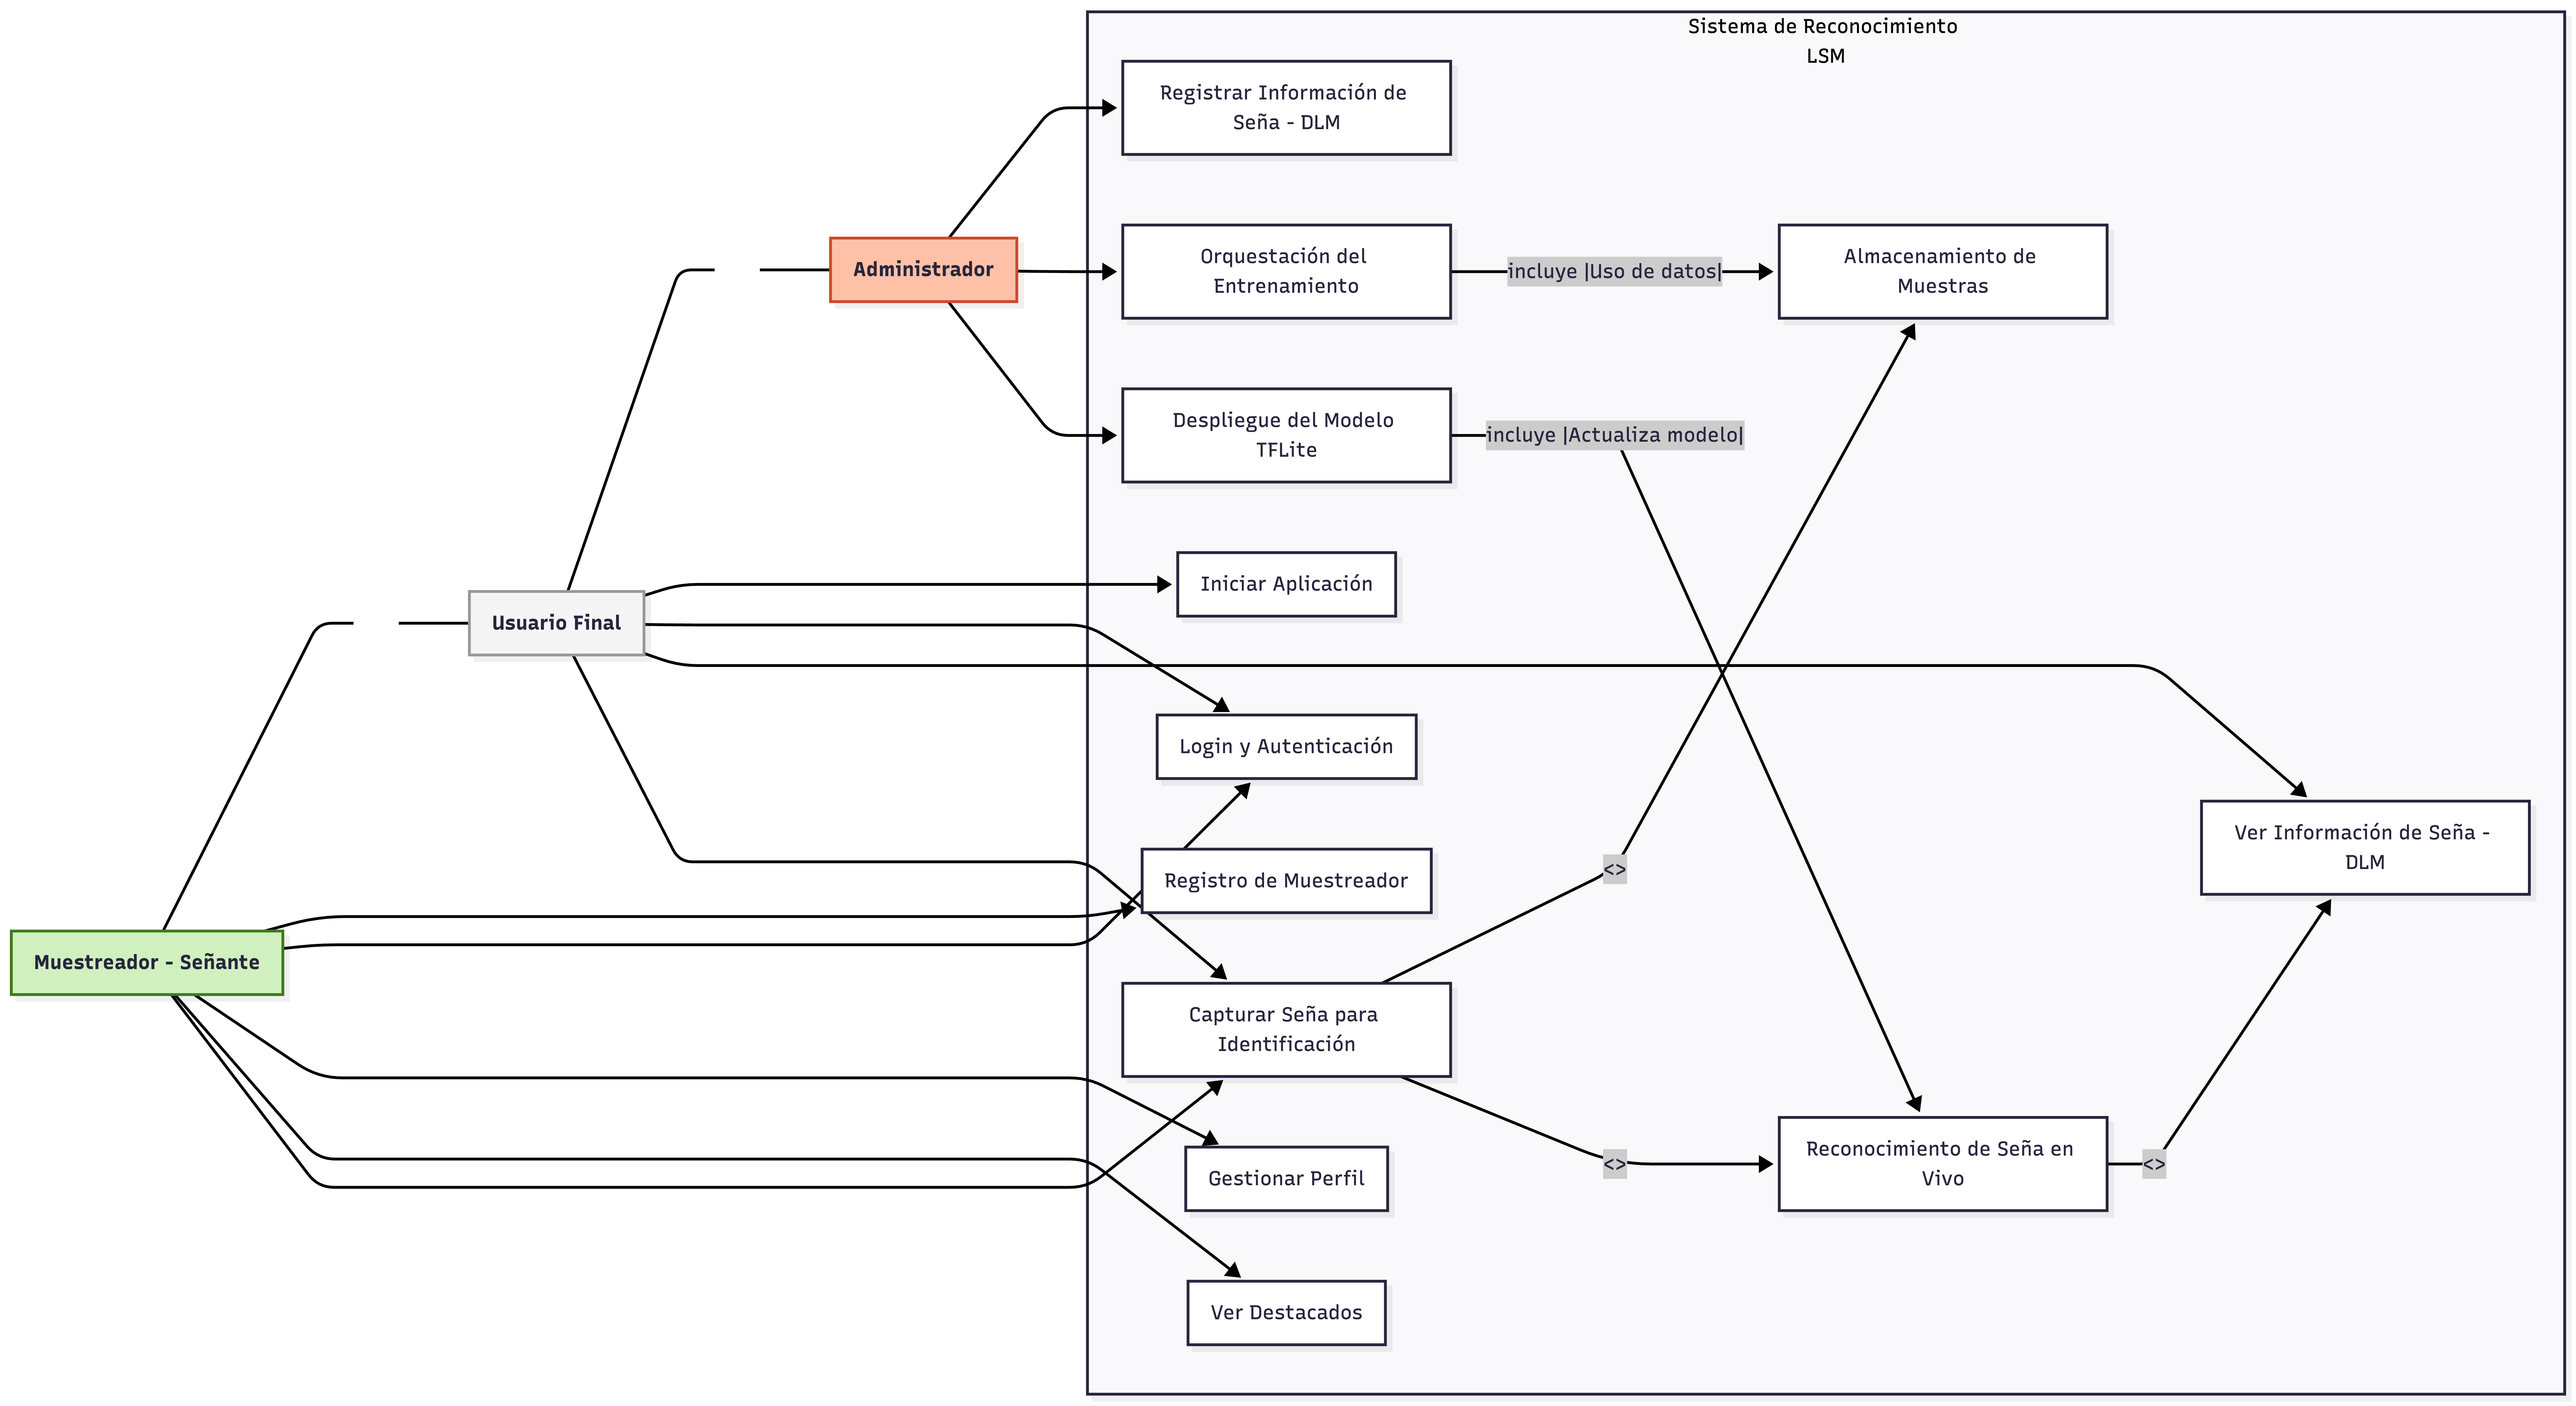
\includegraphics[width=1.2\textwidth]{CAPITULOS/capitulo4/diam}
    \caption{Diagrama de casos de uso del Sistema Principal}
    \label{fig:diagrama_casos_uso}
\end{figure}

\section{Conceptualización y Criterios del Módulo de Machine Learning} \label{sec:conceptualizacion_ml}

Para satisfacer el Requerimiento Funcional de Reconocimiento de Seña (RF08) y, especialmente, los Requerimientos No Funcionales de rendimiento (RNF01 y RNF02), se definió la arquitectura del módulo de clasificación en la fase de análisis. Este módulo se centra en la correcta interpretación de secuencias temporales de datos.

\subsection{Procesamiento de Secuencias y Arquitectura Bi-LSTM}
La Lengua de Señas Mexicana es una lengua visogestual con una fuerte dependencia del movimiento. Por ello, el algoritmo de Machine Learning debe ser capaz de procesar \textbf{secuencias de datos de longitud variable}. La decisión se centra en la justificación que sigue:

\begin{itemize}
    \item \textbf{Normalización Temporal:} Para estandarizar la duración de la seña, se implementa un \textbf{canal de progreso temporal} (ver función \texttt{\_time\_progress\_from\_ts} en \texttt{data\_processor.py}). Esta característica, añadida a los \textit{keypoints} de MediaPipe, permite al modelo Bi-LSTM aprender dónde se encuentra cada \textit{frame} dentro del ciclo de la seña (ej. inicio, articulación, final).
    \item \textbf{Arquitectura Recurrente:} Se selecciona una red \textbf{Bidirectional Long Short-Term Memory (Bi-LSTM)}, tal como se construye en \texttt{model\_constructor.py}. Esta elección es crucial, ya que permite que el modelo analice la secuencia de \textit{keypoints} tanto hacia adelante como hacia atrás, maximizando la comprensión del contexto espacial y temporal de la seña.
    \item \textbf{Técnica de Masking:} La capa \texttt{Masking} se añade en la entrada de la red para manejar secuencias de longitud variable, asegurando que los datos de relleno (\textit{padding}) sean ignorados durante el entrenamiento y la inferencia, lo cual es vital para la precisión.
\end{itemize}

\subsection{Criterios de Despliegue (Edge Computing)}
Dado el RNF02 (Latencia de < 300ms), el modelo debe ser desplegado en el dispositivo (Edge). Los criterios de diseño derivados de este requerimiento son:

\begin{enumerate}
    \item \textbf{Formato TFLite:} El modelo entrenado debe ser convertido al formato optimizado \textbf{TensorFlow Lite (TFLite)} para su ejecución eficiente en el dispositivo Android (\texttt{LiveRecognitionActivity.kt}).
    \item \textbf{Compatibilidad:} La arquitectura Bi-LSTM se construye con capas que aseguran la compatibilidad del grafo con el intérprete de TFLite, evitando operaciones complejas que no se soportan en el despliegue de borde.
\end{enumerate}

\section{Comparación de Tecnologías y Plataformas}

En esta sección se presenta un análisis comparativo integral de las principales tecnologías, plataformas y herramientas consideradas para el diseño e implementación del sistema de reconocimiento de señas. El propósito de esta comparación es evaluar, desde un punto de vista técnico y económico, las distintas alternativas disponibles en cada capa de la arquitectura, con el fin de fundamentar de manera objetiva las decisiones adoptadas en el proyecto.

El análisis abarca múltiples dimensiones del sistema, incluyendo servicios de bases de datos, opciones de cómputo (máquinas virtuales y orquestación de contenedores), almacenamiento de objetos, arquitecturas sin servidor (Function as a Service), APIs de Text-to-Speech, frameworks de aprendizaje automático, arquitecturas de redes neuronales para reconocimiento de secuencias, herramientas de infraestructura como código (IaaS), así como lenguajes y frameworks tanto para el backend como para la aplicación cliente.

Cada subsección presenta una comparación entre las soluciones más relevantes del mercado —principalmente AWS, Google Cloud y Microsoft Azure, junto con alternativas locales y frameworks de software— destacando sus ventajas, limitaciones, costos y grado de adecuación a los requerimientos específicos del proyecto. Finalmente, para cada categoría analizada, se justifica la elección de la tecnología seleccionada, asegurando coherencia arquitectónica, optimización de costos y cumplimiento de los requerimientos funcionales y de rendimiento del sistema.

\subsection{Comparación base de datos en la nube}
En la \textbf{Tabla \ref{tabla_comparativa_plataformas_nube}} se presenta una comparativa de las principales plataformas de nube consideradas para el desarrollo del proyecto, junto con las bases de datos que ofrecen, sus principales usos y su idoneidad para el procesamiento de datos de LSM.

\begin{table}[H]
    \centering
    \caption{Comparación de características entre diferentes plataformas de nube.}
    \label{tabla_comparativa_plataformas_nube}
    \begin{tabularx}{\textwidth}{|>{\raggedright\arraybackslash}p{1cm}|>{\raggedright\arraybackslash}p{2cm}|>{\raggedright\arraybackslash}X|>{\centering\arraybackslash}X|>{\raggedright\arraybackslash}X|}
        \hline
        \textbf{Nube} & \textbf{Base de datos} & \textbf{Ventajas} & \textbf{Costos} & \textbf{Principales usos} \\
        \hline
        AWS & Amazon DynamoDB &
        \begin{itemize}
            \item Amplia gama de servicios
            \item Escalabilidad
            \item Integración con servicios de IA
            \item Base de datos NoSQL
            \item Sin servidor
        \end{itemize} &
        \begin{minipage}[t]{\linewidth}
            Variable\\
            Costo total mensual: \$26.14 USD\\
            Costo por petición de lectura: \$1.05023e-08 USD\\
            Costo por petición de escritura: \$2.22412e-08 USD
        \end{minipage} &
        \begin{itemize}
            \item Cómputo
            \item Almacenamiento
            \item Machine Learning
        \end{itemize} \\
        \hline
        GCP & Cloud SQL &
        \begin{itemize}
            \item Escalabilidad
            \item Integración con TensorFlow
            \item Base de datos relacional
        \end{itemize} &
        \begin{minipage}[t]{\linewidth}
            Variable\\
            Usando MySQL \\
            Arquitectura VM \\
            db-f1-micro \\
            vCPUs: 1\\
            RAM: 3.75 GiB \\
            Costo total mensual: \$24.665 USD
        \end{minipage} &
        \begin{itemize}
            \item Big Data
            \item Machine Learning
        \end{itemize} \\
        \hline
        GCP & Firebase &
        \begin{itemize}
            \item Fácil integración con aplicaciones móviles y web
            \item Soporte para desarrollo rápido de apps
            \item Base de datos NoSQL
        \end{itemize} & Freemium &
        \begin{itemize}
            \item Desarrollo de apps móviles
            \item Desarrollo web
            \item Almacenamiento en la nube
        \end{itemize} \\
        \hline
        Azure & Azure SQL Database &
        \begin{itemize}
            \item Integración con herramientas de Microsoft
            \item Facilidad de uso
            \item Base de datos relacional
        \end{itemize} & Variable &
        \begin{itemize}
            \item Aplicaciones empresariales
            \item Bases de datos
            \item Infraestructura
        \end{itemize} \\
        \hline
    \end{tabularx}
\end{table}

\paragraph{Justificación de la Elección: Amazon DynamoDB}
es la que se ha decidió utilizar como la base de datos principal del sistema. Esta elección se basa en la necesidad de mantener una arquitectura unificada y optimizada, ya que DynamoDB es la solución NoSQL nativa de AWS, la plataforma cloud seleccionada para el despliegue de la aplicación. Su naturaleza sin servidor y su alta escalabilidad permiten una integración fluida con los demás servicios de AWS, como Lambda y S3, ofreciendo un rendimiento predecible y costos eficientes que no dependen solo del cálculo de la máquina virtual (VM), sino del consumo real de peticiones, lo cual es ideal para una aplicación con cargas de trabajo variables.

\subsection{Comparación de VM y Kubernetes de GKE}

En la \textbf{Tabla \ref{tabla_comparativa_microservicios}} se presenta una comparativa de las principales opciones de alojamiento, incluyendo Máquinas Virtuales (VM) y soluciones de contenedores gestionados (como Kubernetes de GKE, EKS y AKS), ofrecidas por las principales plataformas de nube.

\begin{table}[H]
    \centering
    \caption{Comparación de opciones para alojar microservicios en diferentes plataformas de nube.}
    \label{tabla_comparativa_microservicios}
    \begin{tabular}{|p{2.3cm}|p{1.3cm}|p{6cm}|p{6cm}|}
        \hline
        \textbf{Servicio} & \textbf{Nube} & \textbf{Ventajas} & \textbf{Costos} \\
        \hline
        Amazon EC2 & AWS &
        \begin{minipage}[t]{\linewidth}
            \begin{itemize}
                \item Variedad de tipos de instancias para diferentes cargas de trabajo
                \item Escalabilidad automática y opciones de balanceo de carga
                \item Integración con el ecosistema de AWS (RDS, S3, IAM, etc.)
            \end{itemize}
        \end{minipage} &
        % COSTOS AJUSTADOS PARA USO MÍNIMO (10 HORAS)
        \begin{minipage}[t]{\linewidth}
            Costo estimado (\textbf{Instancia Spot}): \textbf{\$10.00 - \$16.00 USD/mes} (aprox.)\\
            Costo basado en \textbf{10 horas de uso activo} de la instancia \textbf{G4dn.xlarge} (GPU):
            \begin{itemize}
                \item vCPUs: 4
                \item Memoria: 16 GiB
                \item GPU: 1 NVIDIA T4
            \end{itemize}
        \end{minipage}
        \\
        \hline
        Amazon EKS & AWS &
        \begin{minipage}[t]{\linewidth}
            \begin{itemize}
                \item Kubernetes gestionado con alta disponibilidad
                \item Fácil integración con otros servicios de AWS
            \end{itemize}
        \end{minipage} &
        \begin{minipage}[t]{\linewidth}
            Costo mensual estimado: \$365.00 USD por mes
            \begin{itemize}
                \item 1 clúster
            \end{itemize}
        \end{minipage} \\
        \hline
        Google Compute Engine (GCE) & Google Cloud &
        \begin{minipage}[t]{\linewidth}
            \begin{itemize}
                \item Alto rendimiento y opciones de personalización
                \item Escalabilidad automática y soporte de GPU/TPU
                \item Integración nativa con GKE para contenedores
            \end{itemize}
        \end{minipage} &
        \begin{minipage}[t]{\linewidth}
            Costo mensual estimado: \$5.55 USD
            \begin{itemize}
                \item Tiempo total de uso de la instancia: 730 horas/mes
                \item Sistema operativo/software: Ubuntu
                \item Tipo de máquina: f1-micro (familia de propósito general, serie N1) con 1 vCPU y 0.9 GiB de RAM
            \end{itemize}
        \end{minipage} \\
        \hline
        Google Kubernetes Engine (GKE) & Google Cloud &
        \begin{minipage}[t]{\linewidth}
            \begin{itemize}
                \item Kubernetes gestionado con escalabilidad automática
                \item Integración con el ecosistema de Google Cloud (BigQuery, Pub/Sub, etc.)
            \end{itemize}
        \end{minipage} &
        \begin{minipage}[t]{\linewidth}
            Costo Mensual estimado: \$152.55 USD
            Coste base por clúster, más recursos usados:
            \begin{itemize}
                \item Machine Family: GP Series:
                \item N1 Machine: f1-micro
            \end{itemize}
        \end{minipage} \\
        \hline
        Azure Virtual Machines & Microsoft Azure &
        \begin{minipage}[t]{\linewidth}
            \begin{itemize}
                \item Integración con otros servicios de Microsoft (Active Directory, SQL Server)
                \item Amplia variedad de opciones de instancias y series
                \item Alta disponibilidad con zonas de disponibilidad
            \end{itemize}
        \end{minipage} &
        \begin{minipage}[t]{\linewidth}
            Costo mensual estimado: \$14.60
            \begin{itemize}
                \item Instancia: A0 (1 núcleo, 0.75 GB RAM) - \$0.020/hora
                \item Sistema operativo: Windows (licencia incluida)

            \end{itemize}
        \end{minipage} \\
        \hline
        Azure Kubernetes Service (AKS) & Microsoft Azure &
        \begin{minipage}[t]{\linewidth}
            \begin{itemize}
                \item Kubernetes gestionado con integración nativa en Azure
                \item Escalabilidad automática de pods y nodos
            \end{itemize}
        \end{minipage} &
        \begin{minipage}[t]{\linewidth}
            Costo mensual estimado: \$158.41\\
            Nodos:
            \begin{itemize}
                \item Sistema operativo: Linux
                \item Instancia: D2 v3 (2 vCPUs, 8 GB RAM) - \$0.117/hora \\
            \end{itemize}

        \end{minipage} \\
        \hline
    \end{tabular}
\end{table}

\textbf{Justificación de la Elección: Amazon EC2 G4dn.xlarge (Spot)}

La elección de la instancia \textbf{Amazon EC2 G4dn.xlarge} mediante el modelo de precios \textbf{Spot} se fundamenta en los requerimientos específicos del proyecto. El \textbf{modelo de Machine Learning} basado en una arquitectura de \textbf{red neuronal recurrente (BiLSTM)} para el reconocimiento de señas requiere de una aceleración de hardware intensiva, lo cual justifica el uso de una Unidad de Procesamiento Gráfico (\textbf{GPU}).

Esta decisión técnica se sustenta en tres pilares clave:
\begin{enumerate}[label=\arabic*., nosep, itemsep=0pt]
    \item \textbf{Requerimiento de GPU:} La G4dn.xlarge proporciona una GPU NVIDIA T4, esencial para acelerar el procesamiento de \textbf{inferencia} del modelo y asegurar la baja latencia necesaria para las pruebas en tiempo real, incluso con uso esporádico.
    \item \textbf{Optimización Extrema de Costos:} Dado que el tiempo de ejecución es \textbf{extremadamente limitado (aproximadamente 10 horas al mes)}, utilizar el modelo Spot reduce el costo por hora de cómputo (GPU intensivo) a su mínima expresión. El costo mensual resultante es bajo, ya que solo cubre una pequeña fracción de horas de cómputo variable y la tarifa base fija por el \textbf{almacenamiento persistente (EBS)} de los 80 GB.
    \item \textbf{Simplicidad Arquitectónica:} La \textbf{Máquina Virtual dedicada (EC2)} simplifica la arquitectura y la gestión operativa para un uso de tan bajo volumen, evitando la complejidad y el costo base fijo de un clúster de orquestación de contenedores (EKS o GKE).
\end{enumerate}
\clearpage

\subsection{Comparación de los servicios de almacenamiento (Bucket)}
En la \textbf{Tabla \ref{tabla_comparativa_buckets}} se presenta una comparativa de las principales opciones de alojamiento de objetos (buckets) ofrecidas por las plataformas de nube.

\vspace{-0.2cm} % <--- AÑADIDO PARA REDUCIR ESPACIO VERTICAL ANTES DE LA TABLA

\begin{table}[H]
    \centering
    \caption{Comparación de servicios de almacenamiento de buckets en diferentes plataformas de nube.}
    \label{tabla_comparativa_buckets}
    \begin{tabular}{|p{1.3cm}|p{1.3cm}|p{4.5cm}|p{4.5cm}|p{4cm}|}
        \hline
        \textbf{Nube} & \textbf{Bucket} & \textbf{Ventajas} & \textbf{Costos} & \textbf{Principales usos} \\
        \hline
        AWS & Amazon S3 &
        \begin{minipage}[t]{\linewidth}
            \begin{itemize}
                \item Alta escalabilidad y durabilidad
                \item Seguridad avanzada (cifrado automático y políticas de acceso granular)
                \item Integración con servicios de AWS (Machine Learning, RedShift, etc.)
                \item Amplia documentación y soporte
            \end{itemize}
        \end{minipage} &
        \begin{minipage}[t]{\linewidth}
            \begin{itemize}
                \item \textbf{Almacenamiento:} \$115.01 USD (5 TB mensuales en S3 Standard)
                \item \textbf{S3 Select:} \$0.0028 USD (datos devueltos), \$0.008 USD (datos escaneados).
                \item \textbf{Total:} \$115.01 USD mensuales (incluyendo S3 Standard, solicitudes de datos y S3 Select).
            \end{itemize}
        \end{minipage} &
        \begin{minipage}[t]{\linewidth}
            \begin{itemize}
                \item Almacenamiento de datos y multimedia
                \item Backup y recuperación ante desastres
                \item Análisis de grandes volúmenes de datos
            \end{itemize}
        \end{minipage} \\
        \hline
        Google Cloud & Google Cloud Storage &
        \begin{minipage}[t]{\linewidth}
            \begin{itemize}
                \item Rendimiento optimizado para grandes datos
                \item Cifrado automático y opciones avanzadas de seguridad
                \item Integración con BigQuery y otras herramientas de análisis de datos
                \item Disponibilidad global con opciones de redundancia
            \end{itemize}
        \end{minipage} &
        \begin{minipage}[t]{\linewidth}
            \begin{itemize}
                \item \textbf{Almacenamiento:} \$99.90 USD (5 TB mensuales en Standard Storage).
                \item \textbf{Transferencias de datos:} Ingreso gratuito, salida desde \$0.12/GB.
                \item \textbf{Operaciones:} \$0.005 por 10,000 operaciones de clase A.
            \end{itemize}
        \end{minipage} &
        \begin{minipage}[t]{\linewidth}
            \begin{itemize}
                \item Almacenamiento de datos
                \item Entrenamiento de modelos de Machine Learning
                \item Archivado y recuperación
                \item Análisis de grandes volúmenes de datos
            \end{itemize}
        \end{minipage} \\
        \hline
        Microsoft Azure & Azure Blob Storage &
        \begin{minipage}[t]{\linewidth}
            \begin{itemize}
                \item Integración con ecosistema de Microsoft (Office, Power BI, etc.)
                \item Escalabilidad con opciones de redundancia (LRS, GRS)
                \item Seguridad con cifrado en tránsito y en reposo
                \item Soporte para migraciones híbridas (Azure Arc)
            \end{itemize}
        \end{minipage} &
        \begin{minipage}[t]{\linewidth}
            \begin{itemize}
                \item \textbf{Standard (GPv2):} Hot (\$0.018/GB), Cool (\$0.01/GB), Archive (\$0.002/GB).
                \item \textbf{Premium:} Optimizado para baja latencia, \$0.15/GB.
                \item \textbf{Reservado:} 100 TB (1 año, \$1,545 Hot), 1 PB (1 año, \$15,050).
                \item \textbf{Early Deletion Penalty:} 30 días (Cool), 90 días (Cold), 180 días (Archive).
            \end{itemize}
        \end{minipage} &
        \begin{minipage}[t]{\linewidth}
            \begin{itemize}
                \item Almacenamiento de datos no estructurados
                \item Respaldo y recuperación ante desastres
                \item Analítica avanzada
                \item Archivo de documentos y multimedia
            \end{itemize}
        \end{minipage} \\
        \hline
    \end{tabular}
\end{table}

\paragraph{Justificación de la Elección: Amazon Simple Storage Service (S3)}
Se ha seleccionado \textbf{Amazon S3} como el servicio de almacenamiento de objetos central del sistema. Esta elección se basa principalmente en la necesidad de integración nativa con la infraestructura AWS ya establecida (EC2 y DynamoDB), y la naturaleza crítica de los datos almacenados. S3 será utilizado para almacenar los siguientes activos:

\begin{enumerate}[label=\arabic*., nosep, itemsep=0pt]
    \item \textbf{Datos Crudos del Modelo (CSV de Keypoints):} Los archivos CSV que contienen las secuencias temporales de Keypoints, que son la materia prima para el entrenamiento y la inferencia del modelo BiLSTM, requieren la \textbf{durabilidad de 99.999999999\%} que ofrece S3 Standard para garantizar la integridad y persistencia de los datos del proyecto.
    \item \textbf{Modelo Compilado:} El archivo del modelo de red neuronal entrenado debe estar disponible con alta fiabilidad para ser cargado por la instancia EC2 (\textbf{G4dn.xlarge}), beneficiándose de la baja latencia de acceso.
    \item \textbf{Archivos de Perfil de Usuario:} Incluyendo fotos de perfil y otros archivos no estructurados que requieran seguridad y fácil gestión de acceso.
\end{enumerate}

La integración nativa de S3 con AWS IAM (para políticas de seguridad) y la facilidad de conexión con la capa de cómputo hacen de esta opción la más eficiente y coherente para la arquitectura del proyecto.

\subsection{Comparación de Function as a Service (FaaS)}

En la \textbf{Tabla \ref{tabla_comparativa_faas}} se presenta una comparativa de los servicios de Function as a Service (FaaS) en las principales plataformas de nube, incluyendo el modelo de costos basado en el consumo.

\begin{table}[H]
    \centering
    \caption{Comparación de Function as a Service en diferentes plataformas de nube.}
    \label{tabla_comparativa_faas}
    \begin{tabular}{|p{1.5cm}|p{1.5cm}|p{4.5cm}|p{5cm}|p{3cm}|} % Se ajustaron los anchos de columna
        \hline
        \textbf{Nube} & \textbf{FaaS} & \textbf{Ventajas} & \textbf{Costo Estimado (por 1 millón de peticiones)} & \textbf{Lenguajes Soportados} \\
        \hline
        AWS & AWS Lambda &
        \begin{minipage}[t]{\linewidth}
            \begin{itemize}
                \item Escalabilidad automática
                \item Integración nativa con DynamoDB, S3 y API Gateway.
                \item Pago por uso.
            \end{itemize}
        \end{minipage} &
        \begin{minipage}[t]{\linewidth}
            \textbf{Aprox. \$2.00 - \$4.00 USD} (Cálculo basado en solicitudes y GB-segundos, posterior a la capa gratuita).
        \end{minipage} &
        \begin{minipage}[t]{\linewidth}
            \begin{itemize}
                \item Python, Node.js, Java, Ruby
            \end{itemize}
        \end{minipage} \\
        \hline
        Google Cloud & Cloud Functions &
        \begin{minipage}[t]{\linewidth}
            \begin{itemize}
                \item Escalabilidad y seguridad
                \item Integración con Google Cloud
            \end{itemize}
        \end{minipage} &
        \begin{minipage}[t]{\linewidth}
            \textbf{Aprox. \$2.50 - \$4.50 USD} (Similar a AWS, posterior a la capa gratuita).
        \end{minipage} &
        \begin{minipage}[t]{\linewidth}
            \begin{itemize}
                \item Node.js, Python, Go
            \end{itemize}
        \end{minipage} \\
        \hline
        Microsoft Azure & Azure Functions &
        \begin{minipage}[t]{\linewidth}
            \begin{itemize}
                \item Integración con servicios de Microsoft
                \item Buen soporte para CI/CD
            \end{itemize}
        \end{minipage} &
        \begin{minipage}[t]{\linewidth}
            \textbf{Aprox. \$2.20 - \$4.20 USD} (Basado en el plan de consumo, posterior a la capa gratuita).
        \end{minipage} &
        \begin{minipage}[t]{\linewidth}
            \begin{itemize}
                \item C\#, JavaScript, Python, Java
            \end{itemize}
        \end{minipage} \\
        \hline
    \end{tabular}
\end{table}

\paragraph{Justificación de la Elección: AWS Lambda}
La selección de \textbf{AWS Lambda} se alinea con la estrategia de mantener una arquitectura de nube unificada en AWS (junto a DynamoDB, S3 y EC2). Lambda es la elección óptima para desacoplar y orquestar las tareas del backend sin incurrir en costos de cómputo inactivos, con un \textbf{costo marginal por petición muy bajo} una vez agotada la generosa capa gratuita.

El diseño del sistema requiere la implementación de \textbf{cuatro funciones Lambda} distintas para manejar responsabilidades específicas, asegurando la escalabilidad e independencia de cada proceso:

\begin{enumerate}[label=\arabic*., nosep, itemsep=0pt]
    \item \textbf{Gestión de Autenticación/Usuarios:} Manejo de registro, inicio de sesión y validación de tokens de usuario.
    \item \textbf{Control de Datos LSM:} Interacción directa con \textbf{DynamoDB} para consultar y almacenar información de la base de datos (metadatos de las señas y perfiles).
    \item \textbf{Gestión de Archivos (S3 Trigger):} Activada por eventos de \textbf{S3}, como la subida de una nueva foto de perfil o un archivo CSV de entrenamiento, gestionando el acceso y la notificación.
    \item \textbf{Orquestación de la Inferencia (EC2 Trigger):} Encargada de comunicarse con la instancia \textbf{EC2 G4dn.xlarge} para iniciar el proceso de inferencia del modelo BiLSTM cuando se recibe una solicitud de reconocimiento de seña.
\end{enumerate}

Este enfoque permite que cada componente del backend escale de forma independiente, pagando únicamente por los milisegundos de cómputo utilizados por cada una de las cuatro funciones.

\subsection{Comparación de APIs de Text-to-Speech (TTS)}

En la \textbf{Tabla \ref{tabla_comparativa_tts}} se presenta una comparativa de las APIs de Text-to-Speech (TTS) en las principales plataformas de nube y la solución nativa de Android.

\begin{table}[H]
    \centering
    \caption{Comparación de servicios Text-to-Speech (TTS): Soluciones en la nube vs. Solución nativa.}
    \label{tabla_comparativa_tts}
    \begin{tabular}{|p{2.5cm}|p{3cm}|p{4cm}|p{3cm}|p{3cm}|}
        \hline
        \textbf{Plataforma} & \textbf{API de TTS} & \textbf{Características} & \textbf{Idiomas soportados} & \textbf{Costo Estimado} \\
        \hline
        AWS & Amazon Polly &
        \begin{minipage}[t]{\linewidth}
            \begin{itemize}
                \item Voces naturales (Neural TTS)
                \item Opciones de personalización
                \item Soporte SSML
            \end{itemize}
        \end{minipage} &
        Más de 30 &
        \begin{minipage}[t]{\linewidth}
            \textbf{Aprox. \$4.00 USD} por 1 millón de caracteres (TTS Estándar)
        \end{minipage} \\
        \hline
        Google Cloud & Google Text-to-Speech &
        \begin{minipage}[t]{\linewidth}
            \begin{itemize}
                \item Tecnología WaveNet
                \item Personalización con SSML
            \end{itemize}
        \end{minipage} &
        Más de 30 &
        \begin{minipage}[t]{\linewidth}
            \textbf{Aprox. \$4.00 USD} por 1 millón de caracteres (TTS Estándar)
        \end{minipage} \\
        \hline
        Microsoft Azure & Azure Speech &
        \begin{minipage}[t]{\linewidth}
            \begin{itemize}
                \item Soporte de voz neural
                \item Personalización de tonos
            \end{itemize}
        \end{minipage} &
        Más de 40 &
        \begin{minipage}[t]{\linewidth}
            \textbf{Aprox. \$4.00 USD} por 1 millón de caracteres (TTS Estándar)
        \end{minipage} \\
        \hline
        Android Nativo & TextToSpeech &
        \begin{minipage}[t]{\linewidth}
            \begin{itemize}
                \item Ejecución local (client-side)
                \item Latencia mínima (sin red)
                \item Funcionalidad offline
            \end{itemize}
        \end{minipage} &
        Depende del dispositivo &
        \begin{minipage}[t]{\linewidth}
            \textbf{Costo de uso nulo} (Gratuito)
        \end{minipage} \\
        \hline
    \end{tabular}
\end{table}

\paragraph{Justificación de la Elección: API Nativa de Android (TextToSpeech)}
Para la funcionalidad de respuesta de voz, el sistema ha optado por utilizar la API nativa de Android, `android.speech.tts.TextToSpeech`, en lugar de las soluciones basadas en la nube. Esta decisión se fundamenta en la arquitectura client-side (del lado del cliente) de la aplicación y en la optimización de recursos y costos:

\begin{enumerate}[label=\arabic*., nosep, itemsep=0pt]
    \item \textbf{Costo Cero (Free Tier):} El uso de la API nativa de Android no genera costos de transacción, consumo de caracteres o latencia de red, a diferencia de las APIs de nube que, aunque tienen una capa gratuita, comienzan a incurrir en gastos con el aumento de uso.
    \item \textbf{Latencia y Rendimiento:} Al ejecutar la síntesis de voz directamente en el dispositivo (cliente), se elimina la latencia de red asociada con el envío de texto a la nube y la recepción del audio.
\end{enumerate}

\subsection{Comparación de Frameworks de Aprendizaje Automático para Reconocimiento}

En la \textbf{Tabla \ref{tabla_comparativa_frameworks}} se presenta una comparativa de los frameworks de aprendizaje automático más utilizados en tareas de reconocimiento de secuencias y visión.

\begin{table}[H]
    \centering
    \caption{Comparación de frameworks de aprendizaje automático para reconocimiento de secuencias.}
    \label{tabla_comparativa_frameworks}
    \begin{tabular}{|p{1.8cm}|p{2.5cm}|p{6.5cm}|p{5cm}|} % Ajuste de anchos para optimizar el espacio
        \hline
        \textbf{Framework} & \textbf{Compatibilidad} & \textbf{Ventajas} & \textbf{Ecosistema y Uso Típico} \\
        \hline
        TensorFlow &
        Multiplataforma (Linux, macOS, Windows) y móvil (Lite) &
        \begin{itemize}
            \item Amplia comunidad, soporte y madurez industrial.
            \item Alto rendimiento en producción y despliegue masivo.
            \item Arquitectura flexible (gráficos estáticos).
        \end{itemize} &
        \begin{itemize}
            \item Modelado de series temporales (RNN, LSTM).
            \item Despliegue en producción (TF Serving, Lite).
        \end{itemize} \\
        \hline
        Keras &
        API de alto nivel para TensorFlow, PyTorch y Theano &
        \begin{itemize}
            \item Simplificación del desarrollo de redes neuronales (fácil y rápido).
            \item Enfocado en la usabilidad y prototipado rápido.
            \item Interfaz estandarizada e intuitiva.
        \end{itemize} &
        \begin{itemize}
            \item Prototipado y desarrollo de Deep Learning.
            \item Construcción de modelos LSTM y BiLSTM.
        \end{itemize} \\
        \hline
        PyTorch &
        Multiplataforma y soporte nativo para GPUs de Nvidia &
        \begin{itemize}
            \item Modelo de grafo dinámico (fácil de depurar y flexible).
            \item Amplio uso en investigación y desarrollo de algoritmos de vanguardia.
            \item Orientado a objetos y muy pitónico.
        \end{itemize} &
        \begin{itemize}
            \item Reconocimiento de voz y clasificación de imágenes.
            \item Investigación y desarrollo de modelos nuevos.
        \end{itemize} \\
        \hline
        MediaPipe &
        C++, Python, JavaScript (Web), Android, iOS &
        \begin{itemize}
            \item Toolkit especializado en percepción multiplataforma.
            \item Detección eficiente de keypoints 3D de Pose, Manos y Rostro.
            \item Optimizado para aplicaciones en tiempo real y on-device.
        \end{itemize} &
        \begin{itemize}
            \item Extracción de características (Preprocesamiento).
            \item Seguimiento y reconocimiento de gestos.
        \end{itemize} \\
        \hline
        OpenCV &
        Multiplataforma; C++ y Python &
        \begin{itemize}
            \item Biblioteca extensa de algoritmos de visión clásica.
            \item Ideal para aplicaciones en tiempo real.
            \item Compatibilidad con C++ y Python.
        \end{itemize} &
        \begin{itemize}
            \item Detección y seguimiento de objetos.
            \item Manipulación de píxeles (pre-procesamiento de video).
        \end{itemize} \\
        \hline
    \end{tabular}
\end{table}

\paragraph{Justificación de la Elección: Keras, TensorFlow y MediaPipe}
La arquitectura de software se basa en la API de \textbf{Keras} con \textbf{TensorFlow} como backend para el modelo BiLSTM, utilizando \textbf{MediaPipe} como herramienta de extracción de características. Esta decisión estratégica se justifica por:

\begin{enumerate}[label=\arabic*., nosep, itemsep=0pt]
    \item \textbf{Eficiencia en Desarrollo (Keras):} La API de Keras simplifica drásticamente la construcción y el entrenamiento de la arquitectura \textbf{Deep BiLSTM}, reduciendo la complejidad del código y el tiempo de prototipado. Keras permite enfocarse en la estructura del modelo sin manejar el detalle de las operaciones de bajo nivel del grafo.
    \item \textbf{Integración y Despliegue (TensorFlow):} Al utilizar TensorFlow como backend, el modelo se beneficia de un ecosistema maduro y enfocado en la producción. Esto facilita el proceso de guardar el modelo en formatos optimizados para el despliegue y su posterior carga en la instancia \textbf{EC2 G4dn.xlarge} para la fase de inferencia en producción.
    \item \textbf{Herramienta de Entrada (MediaPipe):} La elección de \textbf{MediaPipe} es fundamental, ya que es la única biblioteca capaz de proporcionar de manera eficiente los \textbf{vectores de 195 dimensiones (Keypoints de Pose y Manos)} necesarios como entrada secuencial para el modelo BiLSTM. MediaPipe actúa como la capa de extracción de características críticas para el modelo.
\end{enumerate}
\clearpage

\subsection{Comparación de Arquitecturas para el Reconocimiento de Secuencias}

En la \textbf{Tabla \ref{tabla_comparativa_algoritmos}} se presenta una comparación enfocada en redes neuronales profundas, destacando la evolución hacia la arquitectura seleccionada para este proyecto.

\begin{table}[H]
    \centering
    \caption{Comparación de arquitecturas de aprendizaje profundo para el reconocimiento de gestos y secuencias (LSM).}
    \label{tabla_comparativa_algoritmos}
    \begin{tabular}{|p{2.5cm}|p{4.5cm}|p{4.5cm}|p{4.5cm}|}
        \hline
        \textbf{Arquitectura} & \textbf{Características Principales} & \textbf{Aplicación en Video/Señas} & \textbf{Relevancia para el Proyecto} \\
        \hline
        \textbf{CNN} \newline (Redes Neuronales Convolucionales) &
        \begin{itemize}
            \item Especializadas en procesar datos tipo rejilla (imágenes).
            \item Extraen características \textbf{espaciales} (formas de manos, posición del cuerpo).
        \end{itemize} &
        \begin{itemize}
            \item Base de herramientas como \textit{MediaPipe}.
            \item Procesan cada fotograma de forma individual, sin memoria del pasado.
        \end{itemize} &
        \begin{itemize}
            \item Se utilizan implícitamente en la fase de extracción de características (\textbf{MediaPipe}), pero por sí solas no capturan el movimiento temporal de la seña.
        \end{itemize} \\
        \hline
        \textbf{LSTM} \newline (Long Short-Term Memory) &
        \begin{itemize}
            \item Redes recurrentes con "celdas de memoria" para retener información a largo plazo.
            \item Solucionan el problema de desvanecimiento de gradiente de las RNN simples.
        \end{itemize} &
        \begin{itemize}
            \item Ideales para datos secuenciales (series de tiempo, texto, video).
            \item Analizan el movimiento basándose solo en lo ocurrido en el pasado ($t-1$).
        \end{itemize} &
        \begin{itemize}
            \item Son capaces de aprender la secuencia de una seña, pero tienen limitaciones al no conocer el contexto futuro del gesto en movimientos complejos.
        \end{itemize} \\
        \hline
        \textbf{BiLSTM} \newline (Bidirectional LSTM) &
        \begin{itemize}
            \item \textbf{Arquitectura seleccionada.}
            \item Entrena dos capas LSTM simultáneas: una procesa la secuencia de inicio a fin (Forward) y otra de fin a inicio (Backward).
        \end{itemize} &
        \begin{itemize}
            \item Captura el contexto completo de la secuencia.
            \item Crucial en LSM donde la intención de un movimiento inicial a menudo se clarifica por cómo termina la seña.
        \end{itemize} &
        \begin{itemize}
            \item \textbf{Elección del sistema:} Proporciona la mayor precisión al entender la "coarticulación" de los gestos.
            \item Permite distinguir señas con movimientos similares pero contextos diferentes.
        \end{itemize} \\
        \hline
    \end{tabular}
\end{table}

\paragraph{Justificación de la Elección: Arquitectura Bidirectional LSTM (BiLSTM)}
La arquitectura \textbf{BiLSTM} fue seleccionada como la columna vertebral del modelo de reconocimiento de señas por su superioridad inherente en el manejo de datos secuenciales con dependencia de contexto. Esta justificación se basa en tres puntos clave:

\begin{enumerate}[label=\arabic*., nosep, itemsep=0pt]
    \item \textbf{Captura de Contexto Completo:} A diferencia de la LSTM simple, la BiLSTM procesa la secuencia de \textbf{Keypoints} de dos formas: del inicio al final y del final al inicio. Esto es crucial en la Lengua de Señas Mexicana (LSM), donde el significado de un movimiento inicial (e.g., subir la mano) puede depender de la forma en que el gesto concluye. La BiLSTM tiene acceso a ese contexto "futuro" durante el entrenamiento, mejorando drásticamente la precisión.
    \item \textbf{Manejo de Coarticulación:} La capacidad bidireccional permite a la red modelar la coarticulación de los gestos, es decir, cómo el movimiento de una seña influye o se anticipa al movimiento de la seña siguiente. Esto permite distinguir señas con movimientos muy similares pero con transiciones o terminaciones diferentes.
    \item \textbf{Separación de Responsabilidades (CNN vs. BiLSTM):} Es fundamental notar que el sistema divide las tareas:
    \begin{itemize}[nosep, itemsep=0pt] % Aquí se ajusta el espaciado
        \item Las \textbf{CNN} (a través de \textbf{MediaPipe}) son responsables de la extracción de características espaciales (Keypoints) en cada fotograma.
        \item La \textbf{BiLSTM} es responsable de analizar la \textbf{dimensión temporal} de esos Keypoints a lo largo de la secuencia de tiempo, lo que constituye la verdadera tarea de reconocimiento de la seña.
    \end{itemize}
\end{enumerate}
Este enfoque garantiza que el modelo utilice la herramienta más avanzada para cada fase del procesamiento, optimizando la precisión del sistema final.
\clearpage

\subsection{Comparación de lenguajes y frameworks para IaaS}

En la Tabla \ref{tabla_comparativa_iaas} se presenta una comparativa de los principales lenguajes y frameworks utilizados para la gestión de infraestructura como servicio (IaaS), como AWS CloudFormation, Terraform y el marco de trabajo Serverless Application Model (SAM). Estos frameworks permiten la automatización de la infraestructura en la nube, facilitando la creación, configuración y despliegue de recursos de manera eficiente y escalable.

\begin{table}[H]
    \centering
    \caption{Comparación de lenguajes y frameworks para la gestión de infraestructura como servicio (IaaS).}
    \label{tabla_comparativa_iaas}
    \begin{tabular}{|p{2cm}|p{4.5cm}|p{4cm}|p{4cm}|}
        \hline
        \textbf{Framework / Lenguaje} & \textbf{Plataforma Compatible} & \textbf{Ventajas} & \textbf{Principales Usos} \\
        \hline
        AWS CloudFormation &
        AWS &
        \begin{minipage}[t]{\linewidth}
            \begin{itemize}
                \item Integración nativa con AWS.
                \item Soporte para la gestión de recursos complejos.
                \item Escalabilidad y automatización de infraestructuras.
            \end{itemize}
        \end{minipage} &
        \begin{minipage}[t]{\linewidth}
            \begin{itemize}
                \item Despliegue de infraestructuras completas en AWS.
                \item Gestión de entornos de producción, desarrollo y prueba.
                \item Creación de pilas de recursos (stacks) en AWS.
            \end{itemize}
        \end{minipage} \\
        \hline
        Terraform &
        Multicloud (AWS, Azure, Google Cloud, entre otros) &
        \begin{minipage}[t]{\linewidth}
            \begin{itemize}
                \item Multicloud (compatible con múltiples proveedores).
                \item Declarativo y con amplio soporte de proveedores de nube.
                \item Gestión de infraestructura como código (IaC).
            \end{itemize}
        \end{minipage} &
        \begin{minipage}[t]{\linewidth}
            \begin{itemize}
                \item Gestión de infraestructuras en entornos multicloud.
                \item Definición de infraestructura como código para automatizar el aprovisionamiento.
                \item Creación y mantenimiento de entornos a través de archivos de configuración.
            \end{itemize}
        \end{minipage} \\
        \hline
        AWS SAM (Serverless Application Model) &
        AWS (específicamente para aplicaciones sin servidor) &
        \begin{minipage}[t]{\linewidth}
            \begin{itemize}
                \item Simplificación de aplicaciones sin servidor en AWS.
                \item Integración directa con AWS Lambda y otros servicios sin servidor.
                \item Simplificación del proceso de despliegue con plantillas.
            \end{itemize}
        \end{minipage} &
        \begin{minipage}[t]{\linewidth}
            \begin{itemize}
                \item Despliegue de aplicaciones sin servidor (serverless) en AWS.
                \item Integración de funciones Lambda, API Gateway y DynamoDB.
                \item Simplificación de la gestión de recursos sin servidor y microservicios.
            \end{itemize}
        \end{minipage} \\
        \hline
    \end{tabular}
\end{table}

\paragraph{Justificación de la Elección: AWS CloudFormation}

La elección de \textbf{AWS CloudFormation} como framework principal para la gestión de infraestructura como servicio (IaaS) se fundamenta en su capacidad para proporcionar un control exhaustivo y nativo sobre el ciclo de vida de los recursos dentro de la nube de Amazon Web Services (AWS). Aunque alternativas como Terraform ofrecen un enfoque multicloud y AWS SAM simplifica el serverless, CloudFormation se alinea mejor con los requisitos de un sistema robusto y centrado exclusivamente en AWS, por las siguientes razones:

\begin{enumerate}[label=\arabic*., nosep, itemsep=0pt]
    \item \textbf{Integración Nativa y Profunda:} Al ser una herramienta nativa de AWS, CloudFormation garantiza una integración de primer nivel con todos los servicios de AWS, incluyendo los más recientes y complejos. Esto minimiza los posibles retrasos o incompatibilidades que pueden surgir con herramientas de terceros (como Terraform) al gestionar servicios específicos de AWS.
    \item \textbf{Gestión de Ciclo de Vida del Stack:} Permite manejar colecciones de recursos (denominadas stacks) como una única unidad. Esta característica es vital para entornos de producción y prueba, ya que asegura que la creación, actualización o eliminación de la infraestructura se realice de manera atómica, garantizando la consistencia y reduciendo el riesgo de dejar recursos huérfanos o en estados inconsistentes.
    \item \textbf{Seguridad y Gobernanza:} Las plantillas de CloudFormation se validan y procesan a través de los mecanismos de AWS, lo que facilita la implementación de políticas de seguridad y cumplimiento normativo. La creación de Change Sets permite previsualizar exactamente qué recursos serán modificados antes de aplicar los cambios a la infraestructura, ofreciendo una capa crítica de seguridad operacional.
    \item \textbf{Control de Costos:} Al ser una herramienta declarativa y nativa, CloudFormation proporciona una visión clara de los recursos desplegados dentro de un stack, lo cual es fundamental para el monitoreo y la optimización de costos en la plataforma AWS.
\end{enumerate}

Este enfoque nativo proporciona la estabilidad, el control y la escalabilidad necesarias para gestionar eficientemente la infraestructura que soporta la aplicación de reconocimiento de secuencias.

\clearpage

\subsection{Lenguajes de Programación para el Backend}

Para el desarrollo del backend, se ha optado por un enfoque híbrido que aprovecha las fortalezas de dos lenguajes de programación principales: Python y JavaScript (Node.js). Esta estrategia permite optimizar el rendimiento y la eficiencia de costos en la arquitectura de microservicios de AWS. En la \textbf{Tabla \ref{tabla_comparativa_backend}} se presenta una comparación de los lenguajes de programación considerados para el desarrollo de los microservicios en AWS. Esta comparación es crucial para determinar la distribución de responsabilidades, decidiendo qué lenguaje es más eficiente para el cómputo intensivo del modelo BiLSTM y cuál es mejor para la orquestación del servidor.

\begin{table}[H]
    \centering
    \caption{Comparación de Lenguajes de Programación para Microservicios y Lógica de Negocio (Backend).}
    \label{tabla_comparativa_backend}
    \begin{tabular}{|p{1.8cm}|p{3.5cm}|p{5cm}|p{6cm}|}
        \hline
        \textbf{Lenguaje} & \textbf{Rol en el Proyecto} & \textbf{Ventajas Clave} & \textbf{Relevancia para el Proyecto} \\
        \hline
        \textbf{Python} &
        Lógica del \textbf{Modelo BiLSTM}, Preprocesamiento y Tareas Pesadas (EC2/Lambda) &
        \begin{itemize}[nosep, itemsep=0pt]
            \item Ecosistema robusto de ML (TensorFlow/Keras).
            \item Rapidez de prototipado y depuración.
            \item Legibilidad óptima para manipulación de datos.
        \end{itemize} &
        \textbf{Elegido para el cómputo de inferencia}, ya que simplifica la integración directa con las librerías de Deep Learning, siendo el estándar de la industria. \\
        \hline
        \textbf{JavaScript} \newline (Node.js) &
        Servicios de API Gateway, Enrutamiento y Lógica de Negocio (Lambda/Serverless) &
        \begin{itemize}[nosep, itemsep=0pt]
            \item Alto rendimiento en operaciones I/O (asíncrono).
            \item Ecosistema nativo para AWS Serverless (rápida inicialización).
            \item Curva de aprendizaje baja.
        \end{itemize} &
        \textbf{Elegido para la capa de microservicios}, ofreciendo velocidad y eficiencia en el manejo de peticiones web y la comunicación asíncrona. \\
        \hline
        \textbf{Go (Golang)} &
        Servicios de Alto Rendimiento / Alternativa Serverless &
        \begin{itemize}[nosep, itemsep=0pt]
            \item Lenguaje compilado, alta velocidad y eficiencia en uso de memoria.
            \item Excelente manejo de la concurrencia.
            \item Despliegue de binarios pequeños.
        \end{itemize} &
        \textbf{Descartado:} Aunque es rápido, su ecosistema de Deep Learning es inmaduro comparado con Python, lo que complicaría la integración y el mantenimiento del modelo BiLSTM. \\
        \hline
    \end{tabular}
\end{table}

\paragraph{Justificación del Enfoque Híbrido en el Backend}
La arquitectura de backend utiliza una doble capa para optimizar los recursos. \textbf{JavaScript} se encarga del manejo rápido y asíncrono de las peticiones del \textbf{API Gateway} y la lógica serverless de bajo cómputo, actuando como un orquestador eficiente. Por otro lado, \textbf{Python} es el lenguaje exclusivo para las funciones críticas de \textbf{inferencia del modelo BiLSTM}, garantizando la máxima compatibilidad y rendimiento con las librerías de TensorFlow/Keras. Esta división asegura que cada lenguaje se use para la tarea en la que sobresale, maximizando la eficiencia operativa.

\subsection{Lenguajes de Programación para la Aplicación Cliente}

El desarrollo de la aplicación móvil requiere un lenguaje que asegure el máximo rendimiento y una baja latencia en tareas intensivas como la captura y el procesamiento de video con MediaPipe. En la \textbf{Tabla \ref{tabla_comparativa_client_app}} se analizan las opciones para el desarrollo de la aplicación móvil cliente. La elección se centra en garantizar el máximo rendimiento para las tareas intensivas de video y cámara que requiere la integración con MediaPipe.

\begin{table}[H]
    \centering
    \caption{Comparación de Lenguajes y Frameworks para el Desarrollo de Aplicaciones Cliente.}
    \label{tabla_comparativa_client_app}
    \begin{tabular}{|p{2.5cm}|p{3.5cm}|p{5cm}|p{5.5cm}|}
        \hline
        \textbf{Lenguaje} & \textbf{Plataforma de Despliegue} & \textbf{Ventajas Clave} & \textbf{Desventajas y Decisión} \\
        \hline
        \textbf{Kotlin} &
        Android Nativo / KMM (Multiplataforma) &
        \begin{itemize}[nosep, itemsep=0pt]
            \item Lenguaje moderno, conciso y seguro (minimiza errores de null).
            \item \textbf{Soporte oficial de Google} para el desarrollo de Android.
            \item Excelente interoperabilidad con Java.
        \end{itemize} &
        \textbf{Elección del Cliente:} Proporciona el \textbf{mejor rendimiento nativo} en aplicaciones Android, crucial para el procesamiento en tiempo real de la cámara y la integración eficiente de la capa de MediaPipe. \\
        \hline
        \textbf{Java} &
        Android Nativo (Tradicional) &
        \begin{itemize}[nosep, itemsep=0pt]
            \item Amplia base de código legado y documentación.
            \item Alto rendimiento nativo.
        \end{itemize} &
        Es una alternativa viable, pero el lenguaje es más verboso, requiere más código para las mismas funcionalidades y es menos seguro que Kotlin, lo que aumenta el tiempo de desarrollo. \\
        \hline
        \textbf{React Native} &
        iOS / Android (Híbrido) &
        \begin{itemize}[nosep, itemsep=0pt]
            \item Una sola base de código para ambas plataformas.
            \item Amplia comunidad web.
        \end{itemize} &
        \textbf{Descartado:} No es adecuado debido a la necesidad de rendimiento \textbf{nativo puro} para tareas intensivas como la integración profunda de la cámara y la latencia en el procesamiento de Keypoints, donde las capas puente pueden ser limitantes. \\
        \hline
    \end{tabular}
\end{table}

\paragraph{Justificación de la Elección de Kotlin}
Se seleccionó \textbf{Kotlin} como lenguaje principal para la aplicación cliente debido a que es el estándar moderno y oficialmente preferido por Google para el desarrollo de Android. Esta elección asegura una integración de máximo rendimiento con las APIs del sistema operativo y las librerías nativas de la cámara, un requisito indispensable para la baja latencia exigida por el procesamiento de \textbf{MediaPipe} y la comunicación eficiente con el \textbf{API Gateway} del backend. Esto garantiza una experiencia de usuario fluida y receptiva.

\subsection{Tecnologías Utilizadas}

A continuación, se detallan las principales tecnologías que serán utilizadas para el desarrollo, entrenamiento y despliegue del sistema de reconocimiento de LSM, alineadas con la arquitectura BiLSTM y la infraestructura AWS.

\begin{itemize}[nosep, itemsep=0.7pt]
    \item \textbf{Herramientas Core y Modelado}
    \begin{itemize}[nosep, itemsep=0pt]
        \item \textbf{Python}: Lenguaje de programación principal para la lógica del sistema, pre-procesamiento de datos y el flujo de trabajo de aprendizaje profundo.
        \item \textbf{MediaPipe Holistic}: Módulo clave para la extracción de características espaciales (Keypoints de manos, cuerpo y rostro) en tiempo real, proporcionando las secuencias de entrada para la red BiLSTM.
        \item \textbf{TensorFlow / Keras}: Framework principal de Deep Learning utilizado para construir, entrenar y optimizar la arquitectura de red Bidirectional LSTM (BiLSTM), responsable del análisis de la dimensión temporal.
    \end{itemize}

    \item \textbf{Arquitectura Cloud y Microservicios (AWS)}
    \begin{itemize}[nosep, itemsep=0pt]
        \item \textbf{Amazon API Gateway}: Actúa como el \textbf{punto de entrada unificado} para la interfaz web. Recibe las peticiones de reconocimiento y las enruta a las funciones Lambda correspondientes.
        \item \textbf{AWS Lambda}: Ejecuta el código de inferencia del modelo BiLSTM en un entorno serverless, escalable y bajo demanda, lo cual optimiza los costos operativos.
        \item \textbf{Amazon S3 (Simple Storage Service)}: Almacenamiento escalable de objetos para videos fuente, secuencias de Keypoints pre-procesados y los modelos BiLSTM entrenados.
        \item \textbf{Amazon EC2 (Elastic Compute Cloud)}: Servicio de computación utilizado para desplegar instancias con capacidades de GPU, reservado específicamente para el \textbf{entrenamiento y re-entrenamiento periódico} de los modelos BiLSTM.
        \item \textbf{API de Text-To-Speech (TTS)}: Servicio integrado (posiblemente Amazon Polly) para la generación de feedback de voz al usuario.
    \end{itemize}

    \item \textbf{Gestión Operacional y Seguridad}
    \begin{itemize}[nosep, itemsep=0pt]
        \item \textbf{AWS Secrets Manager}: Utilizado para almacenar y rotar de forma segura credenciales, claves de API y otros secretos sensibles, separándolos del código de la aplicación.
        \item \textbf{AWS Systems Manager (SSM) Client}: Herramienta de gestión de operaciones que facilita el acceso remoto seguro y la automatización de tareas en las instancias EC2, sin exponer puertos de red.
    \end{itemize}

    \item \textbf{Infraestructura como Código (IaC)}
    \begin{itemize}[nosep, itemsep=0pt]
        \item \textbf{AWS CloudFormation}: Servicio fundamental para automatizar el despliegue y la gestión de la infraestructura como código (IaC), manteniendo la consistencia y el control atómico de todos los recursos en la nube.
    \end{itemize}
    \item \textbf{Lenguajes de Programación}
    \begin{itemize}[nosep, itemsep=0pt]
        \item \textbf{Python}: Lenguaje principal para el flujo de trabajo de \textbf{Deep Learning}, el pre-procesamiento de datos y la inferencia del modelo BiLSTM.
        \item \textbf{JavaScript (Node.js)}: Utilizado para la \textbf{capa de microservicios} y el enrutamiento serverless (AWS Lambda), optimizando el rendimiento de las operaciones I/O.
        \item \textbf{Kotlin}: Lenguaje de programación nativo moderno, elegido para el desarrollo de la \textbf{aplicación móvil cliente} para garantizar el máximo rendimiento en el procesamiento de video con MediaPipe.
        \item \textbf{Java}: Utilizado en la aplicación móvil para la interoperabilidad con librerías nativas de Android y para el manejo del SDK, trabajando en conjunto con Kotlin.
    \end{itemize}
\end{itemize}
\clearpage

\section{Análisis de Viabilidad Económica y Costos Operacionales}
La implementación de la arquitectura de Deep Learning y microservicios en la nube conlleva un costo operativo que debe ser estimado para evaluar la viabilidad del proyecto. A continuación, se presenta un análisis de los costos operativos mensuales proyectados, basados en un escenario de uso moderado (piloto) en la plataforma AWS, con un \textbf{costo total estimado de \$41.04 USD por mes}.La figura \ref{fig:costo} ilustra la distribución porcentual de esta inversión, destacando el cómputo como principal factor de gasto.

\begin{figure}[H]
    \centering
    % Se quitó la etiqueta de aquí (ANTES)
    \begin{tikzpicture}
        \pie[
            sum=41.04, % Total actualizado
            text=legend,
            color={red!60, blue!60, green!60, orange!60, gray!60}
        ]{
            21.04/Entrenamiento (EC2/GPU - 51\%), % 51%
            11.50/Almacenamiento (S3 - 28\%), % 28%
            5.00/Inferencia (Lambda - 12\%), % 12%
            2.50/Base de Datos (DynamoDB - 6\%), % 6%
            1.00/Orquestación/Gestión (API GW/CF - 2\%) % 2% (valor y descripción actualizados)
        }
    \end{tikzpicture}
    \caption{Proyección de Costos Mensuales Estimados (Entorno Piloto) en AWS}
    \label{fig:costo} % <<--- SOLUCIÓN: LA ETIQUETA DEBE IR AQUÍ.
\end{figure}

La contención de costos se logra, en gran medida, gracias al aprovechamiento estratégico de la \textbf{Capa Gratuita (Free Tier)} de AWS para servicios como AWS Lambda, API Gateway y DynamoDB, que cubren la mayor parte del uso en el entorno piloto. Asimismo, el uso de herramientas \textbf{Open Source} como Python, TensorFlow y MediaPipe elimina las licencias de software, permitiendo que la inversión se centre casi exclusivamente en los recursos de cómputo y almacenamiento esenciales para el entrenamiento del modelo.

\subsubsection*{Recursos Gratuitos (Zero-Cost) Clave}

El proyecto depende de manera crítica de tecnologías de código abierto o capas gratuitas de servicios en la nube para reducir el gasto operacional inicial. Estos recursos no generan costos de licencia o suscripción:

\begin{itemize}[nosep, itemsep=0pt]
    \item \textbf{Frameworks de Machine Learning y Visión por Computadora (Open Source):}
    \begin{itemize}[nosep, itemsep=0pt]
        \item \textbf{Python}, \textbf{TensorFlow / Keras}: Lenguajes y librerías fundamentales de ML.
        \item \textbf{MediaPipe Holistic}: Módulo clave para la detección de Keypoints de manos y cuerpo.
    \end{itemize}
    \item \textbf{Lenguajes de Aplicación (Open Source):}
    \begin{itemize}[nosep, itemsep=0pt]
        \item \textbf{Kotlin} y \textbf{Java}: Utilizados para el desarrollo de aplicaciones Android.
        \item \textbf{JavaScript (Node.js)}: Utilizado para la lógica serverless y el enrutamiento.
    \end{itemize}
    \item \textbf{Servicios Cloud (Free Tier - Uso Básico):}
    \begin{itemize}[nosep, itemsep=0pt]
        \item \textbf{AWS Lambda} y \textbf{API Gateway}: Cobertura de las primeras ejecuciones y peticiones.
        \item \textbf{Amazon DynamoDB}: Cobertura de almacenamiento de datos y unidades de capacidad.
        \item \textbf{AWS CloudFormation}: Servicio de IaC sin costo directo.
    \end{itemize}
\end{itemize}